\textbf{[What does the GUI want to achieve? High-level point?]}

The user interface of the application focusses\textbf{[sp?]} on the displayed
visualization, which takes up the majority of the window, and can be maximised
to fill the available space. Other panels occupy the right and bottom sections
of the window, and are as follows.

Choice of visualization is presented to the user by a list in the top of the
right panel, followed underneath by options specific to that visualisation, and
then by general filters to refine the processed data. \textbf{[If recorded data is used,]} time controls are
included on the right panel to allow the user to fine-tune the speed at which
data is processed and displayed \textbf{[explain]}. The right panel is ultimately aimed at
providing the user with options to adapt the shown data.

The function of the bottom panel is to show fine and aggregate details of the
processed data. To fit the large amount of data available into such a limited
space, a tabbed pane is used on the left to categorise distinct types of data.
The right section of this panel contains a `Context Pane', the purpose of
which is to show further detail of selected data on demand. The left
`Analysis' panel and the right `Context' panel are split in two by a split
pane, so the user can modify the proportion of each they wish to see. \textbf{[extend this.]}

\textbf{[DP suggests to remove the following paragraphs.]}

Less-frequently used program functions, as well as window tools, are included
in the form of a main menu bar. Common window tasks are available via the menu
bar, as well as an exclusive-mode full screen option and the facility to select
a new data source.

Messages to the user come in the form of warning dialogues for user or program
errors, notifications in the bottom `Analysis' panel for program notifications,
and text messages in the bottom `Context' panel for help messages and
suggestions. A diagram of the application layout is included below.

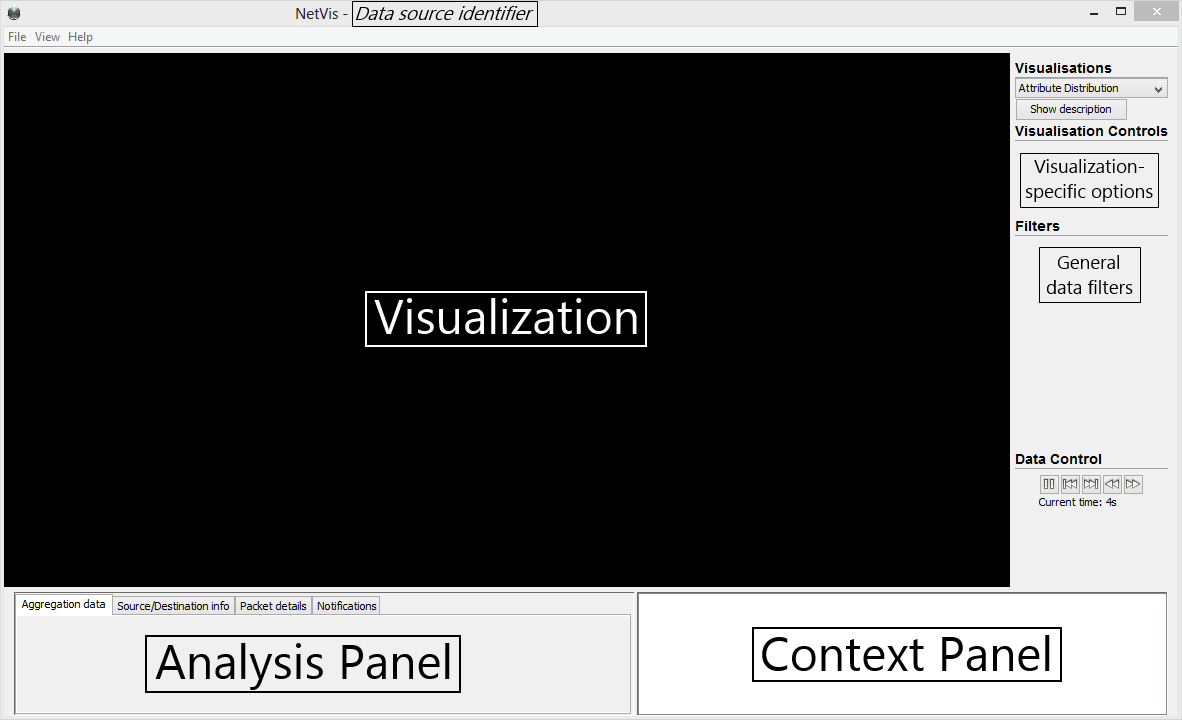
\includegraphics[width=\linewidth]{materials/layout-diagram.png}
